% Graphic for TeX using PGF
% Title: /home/erwan/wip/svn_uima/UIMAv00maq/erwan/dev/rapport/TS/TS06a.dia
% Creator: Dia v0.97.1
% CreationDate: Tue Jan 25 14:06:44 2011
% For: erwan
% \usepackage{tikz}
% The following commands are not supported in PSTricks at present
% We define them conditionally, so when they are implemented,
% this pgf file will use them.
\ifx\du\undefined
  \newlength{\du}
\fi
\setlength{\du}{15\unitlength}
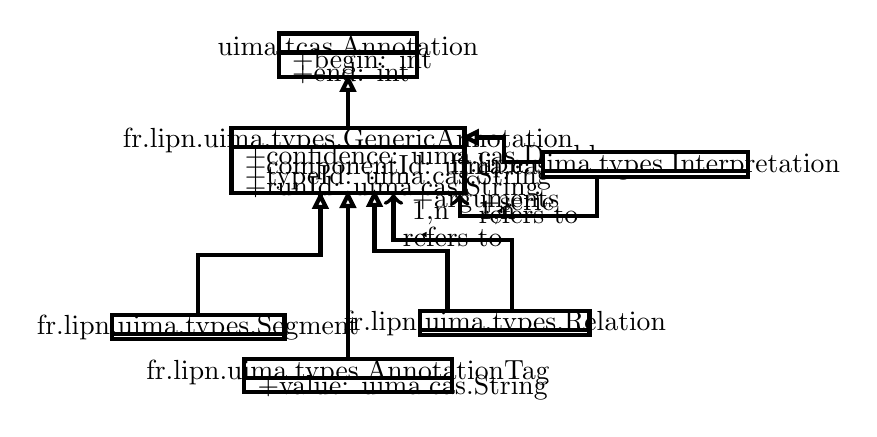
\begin{tikzpicture}
\pgftransformxscale{0.326013}
\pgftransformyscale{-0.326013}
\definecolor{dialinecolor}{rgb}{0.000000, 0.000000, 0.000000}
\pgfsetstrokecolor{dialinecolor}
\definecolor{dialinecolor}{rgb}{1.000000, 1.000000, 1.000000}
\pgfsetfillcolor{dialinecolor}
\pgfsetlinewidth{0.100000\du}
\pgfsetdash{}{0pt}
\definecolor{dialinecolor}{rgb}{1.000000, 1.000000, 1.000000}
\pgfsetfillcolor{dialinecolor}
\fill (20.179400\du,2.400000\du)--(20.179400\du,3.800000\du)--(30.389400\du,3.800000\du)--(30.389400\du,2.400000\du)--cycle;
\definecolor{dialinecolor}{rgb}{0.000000, 0.000000, 0.000000}
\pgfsetstrokecolor{dialinecolor}
\draw (20.179400\du,2.400000\du)--(20.179400\du,3.800000\du)--(30.389400\du,3.800000\du)--(30.389400\du,2.400000\du)--cycle;
% setfont left to latex
\definecolor{dialinecolor}{rgb}{0.000000, 0.000000, 0.000000}
\pgfsetstrokecolor{dialinecolor}
\node at (25.284400\du,3.350000\du){uima.tcas.Annotation};
\definecolor{dialinecolor}{rgb}{1.000000, 1.000000, 1.000000}
\pgfsetfillcolor{dialinecolor}
\fill (20.179400\du,3.800000\du)--(20.179400\du,5.600000\du)--(30.389400\du,5.600000\du)--(30.389400\du,3.800000\du)--cycle;
\definecolor{dialinecolor}{rgb}{0.000000, 0.000000, 0.000000}
\pgfsetstrokecolor{dialinecolor}
\draw (20.179400\du,3.800000\du)--(20.179400\du,5.600000\du)--(30.389400\du,5.600000\du)--(30.389400\du,3.800000\du)--cycle;
% setfont left to latex
\definecolor{dialinecolor}{rgb}{0.000000, 0.000000, 0.000000}
\pgfsetstrokecolor{dialinecolor}
\node[anchor=west] at (20.329400\du,4.500000\du){+begin: int};
% setfont left to latex
\definecolor{dialinecolor}{rgb}{0.000000, 0.000000, 0.000000}
\pgfsetstrokecolor{dialinecolor}
\node[anchor=west] at (20.329400\du,5.300000\du){+end: int};
\pgfsetlinewidth{0.100000\du}
\pgfsetdash{}{0pt}
\definecolor{dialinecolor}{rgb}{1.000000, 1.000000, 1.000000}
\pgfsetfillcolor{dialinecolor}
\fill (16.674400\du,9.380000\du)--(16.674400\du,10.780000\du)--(33.894400\du,10.780000\du)--(33.894400\du,9.380000\du)--cycle;
\definecolor{dialinecolor}{rgb}{0.000000, 0.000000, 0.000000}
\pgfsetstrokecolor{dialinecolor}
\draw (16.674400\du,9.380000\du)--(16.674400\du,10.780000\du)--(33.894400\du,10.780000\du)--(33.894400\du,9.380000\du)--cycle;
% setfont left to latex
\definecolor{dialinecolor}{rgb}{0.000000, 0.000000, 0.000000}
\pgfsetstrokecolor{dialinecolor}
\node at (25.284400\du,10.330000\du){fr.lipn.uima.types.GenericAnnotation};
\definecolor{dialinecolor}{rgb}{1.000000, 1.000000, 1.000000}
\pgfsetfillcolor{dialinecolor}
\fill (16.674400\du,10.780000\du)--(16.674400\du,14.180000\du)--(33.894400\du,14.180000\du)--(33.894400\du,10.780000\du)--cycle;
\definecolor{dialinecolor}{rgb}{0.000000, 0.000000, 0.000000}
\pgfsetstrokecolor{dialinecolor}
\draw (16.674400\du,10.780000\du)--(16.674400\du,14.180000\du)--(33.894400\du,14.180000\du)--(33.894400\du,10.780000\du)--cycle;
% setfont left to latex
\definecolor{dialinecolor}{rgb}{0.000000, 0.000000, 0.000000}
\pgfsetstrokecolor{dialinecolor}
\node[anchor=west] at (16.824400\du,11.480000\du){+confidence: uima.cas.Double};
% setfont left to latex
\definecolor{dialinecolor}{rgb}{0.000000, 0.000000, 0.000000}
\pgfsetstrokecolor{dialinecolor}
\node[anchor=west] at (16.824400\du,12.280000\du){+componentId: uima.cas.String};
% setfont left to latex
\definecolor{dialinecolor}{rgb}{0.000000, 0.000000, 0.000000}
\pgfsetstrokecolor{dialinecolor}
\node[anchor=west] at (16.824400\du,13.080000\du){+typeId: uima.cas.String};
% setfont left to latex
\definecolor{dialinecolor}{rgb}{0.000000, 0.000000, 0.000000}
\pgfsetstrokecolor{dialinecolor}
\node[anchor=west] at (16.824400\du,13.880000\du){+runId: uima.cas.String};
\pgfsetlinewidth{0.100000\du}
\pgfsetdash{}{0pt}
\pgfsetmiterjoin
\pgfsetbuttcap
{
\definecolor{dialinecolor}{rgb}{0.000000, 0.000000, 0.000000}
\pgfsetfillcolor{dialinecolor}
% was here!!!
\definecolor{dialinecolor}{rgb}{0.000000, 0.000000, 0.000000}
\pgfsetstrokecolor{dialinecolor}
\draw (25.284400\du,5.650403\du)--(25.284400\du,5.650403\du)--(25.284400\du,9.329701\du)--(25.284400\du,9.329701\du);
}
\definecolor{dialinecolor}{rgb}{0.000000, 0.000000, 0.000000}
\pgfsetstrokecolor{dialinecolor}
\draw (25.284400\du,6.562206\du)--(25.284400\du,9.329701\du)--(25.284400\du,9.329701\du);
\pgfsetmiterjoin
\definecolor{dialinecolor}{rgb}{1.000000, 1.000000, 1.000000}
\pgfsetfillcolor{dialinecolor}
\fill (25.684400\du,6.562206\du)--(25.284400\du,5.762206\du)--(24.884400\du,6.562206\du)--cycle;
\pgfsetlinewidth{0.100000\du}
\pgfsetdash{}{0pt}
\pgfsetmiterjoin
\definecolor{dialinecolor}{rgb}{0.000000, 0.000000, 0.000000}
\pgfsetstrokecolor{dialinecolor}
\draw (25.684400\du,6.562206\du)--(25.284400\du,5.762206\du)--(24.884400\du,6.562206\du)--cycle;
% setfont left to latex
\pgfsetlinewidth{0.100000\du}
\pgfsetdash{}{0pt}
\pgfsetmiterjoin
\pgfsetbuttcap
{
\definecolor{dialinecolor}{rgb}{0.000000, 0.000000, 0.000000}
\pgfsetfillcolor{dialinecolor}
% was here!!!
\definecolor{dialinecolor}{rgb}{0.000000, 0.000000, 0.000000}
\pgfsetstrokecolor{dialinecolor}
\draw (33.894400\du,10.080000\du)--(36.784700\du,10.080000\du)--(36.784700\du,11.880000\du)--(39.675000\du,11.880000\du);
}
\definecolor{dialinecolor}{rgb}{0.000000, 0.000000, 0.000000}
\pgfsetstrokecolor{dialinecolor}
\draw (34.806203\du,10.080000\du)--(36.784700\du,10.080000\du)--(36.784700\du,11.880000\du)--(39.675000\du,11.880000\du);
\pgfsetmiterjoin
\definecolor{dialinecolor}{rgb}{1.000000, 1.000000, 1.000000}
\pgfsetfillcolor{dialinecolor}
\fill (34.806203\du,9.680000\du)--(34.006203\du,10.080000\du)--(34.806203\du,10.480000\du)--cycle;
\pgfsetlinewidth{0.100000\du}
\pgfsetdash{}{0pt}
\pgfsetmiterjoin
\definecolor{dialinecolor}{rgb}{0.000000, 0.000000, 0.000000}
\pgfsetstrokecolor{dialinecolor}
\draw (34.806203\du,9.680000\du)--(34.006203\du,10.080000\du)--(34.806203\du,10.480000\du)--cycle;
% setfont left to latex
\pgfsetlinewidth{0.100000\du}
\pgfsetdash{}{0pt}
\pgfsetmiterjoin
\pgfsetbuttcap
{
\definecolor{dialinecolor}{rgb}{0.000000, 0.000000, 0.000000}
\pgfsetfillcolor{dialinecolor}
% was here!!!
\definecolor{dialinecolor}{rgb}{0.000000, 0.000000, 0.000000}
\pgfsetstrokecolor{dialinecolor}
\draw (27.250000\du,14.150000\du)--(27.250000\du,18.466250\du)--(32.634450\du,18.466250\du)--(32.634450\du,22.782500\du);
}
\definecolor{dialinecolor}{rgb}{0.000000, 0.000000, 0.000000}
\pgfsetstrokecolor{dialinecolor}
\draw (27.250000\du,15.061803\du)--(27.250000\du,18.466250\du)--(32.634450\du,18.466250\du)--(32.634450\du,22.782500\du);
\pgfsetmiterjoin
\definecolor{dialinecolor}{rgb}{1.000000, 1.000000, 1.000000}
\pgfsetfillcolor{dialinecolor}
\fill (27.650000\du,15.061803\du)--(27.250000\du,14.261803\du)--(26.850000\du,15.061803\du)--cycle;
\pgfsetlinewidth{0.100000\du}
\pgfsetdash{}{0pt}
\pgfsetmiterjoin
\definecolor{dialinecolor}{rgb}{0.000000, 0.000000, 0.000000}
\pgfsetstrokecolor{dialinecolor}
\draw (27.650000\du,15.061803\du)--(27.250000\du,14.261803\du)--(26.850000\du,15.061803\du)--cycle;
% setfont left to latex
\pgfsetlinewidth{0.100000\du}
\pgfsetdash{}{0pt}
\definecolor{dialinecolor}{rgb}{1.000000, 1.000000, 1.000000}
\pgfsetfillcolor{dialinecolor}
\fill (17.625000\du,26.475000\du)--(17.625000\du,27.875000\du)--(32.942500\du,27.875000\du)--(32.942500\du,26.475000\du)--cycle;
\definecolor{dialinecolor}{rgb}{0.000000, 0.000000, 0.000000}
\pgfsetstrokecolor{dialinecolor}
\draw (17.625000\du,26.475000\du)--(17.625000\du,27.875000\du)--(32.942500\du,27.875000\du)--(32.942500\du,26.475000\du)--cycle;
% setfont left to latex
\definecolor{dialinecolor}{rgb}{0.000000, 0.000000, 0.000000}
\pgfsetstrokecolor{dialinecolor}
\node at (25.283750\du,27.425000\du){fr.lipn.uima.types.AnnotationTag};
\definecolor{dialinecolor}{rgb}{1.000000, 1.000000, 1.000000}
\pgfsetfillcolor{dialinecolor}
\fill (17.625000\du,27.875000\du)--(17.625000\du,28.875000\du)--(32.942500\du,28.875000\du)--(32.942500\du,27.875000\du)--cycle;
\definecolor{dialinecolor}{rgb}{0.000000, 0.000000, 0.000000}
\pgfsetstrokecolor{dialinecolor}
\draw (17.625000\du,27.875000\du)--(17.625000\du,28.875000\du)--(32.942500\du,28.875000\du)--(32.942500\du,27.875000\du)--cycle;
% setfont left to latex
\definecolor{dialinecolor}{rgb}{0.000000, 0.000000, 0.000000}
\pgfsetstrokecolor{dialinecolor}
\node[anchor=west] at (17.775000\du,28.575000\du){+value: uima.cas.String};
\pgfsetlinewidth{0.100000\du}
\pgfsetdash{}{0pt}
\pgfsetmiterjoin
\pgfsetbuttcap
{
\definecolor{dialinecolor}{rgb}{0.000000, 0.000000, 0.000000}
\pgfsetfillcolor{dialinecolor}
% was here!!!
\definecolor{dialinecolor}{rgb}{0.000000, 0.000000, 0.000000}
\pgfsetstrokecolor{dialinecolor}
\draw (25.284400\du,14.230299\du)--(25.284400\du,20.327497\du)--(25.283750\du,20.327497\du)--(25.283750\du,26.424695\du);
}
\definecolor{dialinecolor}{rgb}{0.000000, 0.000000, 0.000000}
\pgfsetstrokecolor{dialinecolor}
\draw (25.284400\du,15.142102\du)--(25.284400\du,20.327497\du)--(25.283750\du,20.327497\du)--(25.283750\du,26.424695\du);
\pgfsetmiterjoin
\definecolor{dialinecolor}{rgb}{1.000000, 1.000000, 1.000000}
\pgfsetfillcolor{dialinecolor}
\fill (25.684400\du,15.142102\du)--(25.284400\du,14.342102\du)--(24.884400\du,15.142102\du)--cycle;
\pgfsetlinewidth{0.100000\du}
\pgfsetdash{}{0pt}
\pgfsetmiterjoin
\definecolor{dialinecolor}{rgb}{0.000000, 0.000000, 0.000000}
\pgfsetstrokecolor{dialinecolor}
\draw (25.684400\du,15.142102\du)--(25.284400\du,14.342102\du)--(24.884400\du,15.142102\du)--cycle;
% setfont left to latex
\pgfsetlinewidth{0.100000\du}
\pgfsetdash{}{0pt}
\definecolor{dialinecolor}{rgb}{1.000000, 1.000000, 1.000000}
\pgfsetfillcolor{dialinecolor}
\fill (7.823750\du,23.182500\du)--(7.823750\du,24.582500\du)--(20.593750\du,24.582500\du)--(20.593750\du,23.182500\du)--cycle;
\definecolor{dialinecolor}{rgb}{0.000000, 0.000000, 0.000000}
\pgfsetstrokecolor{dialinecolor}
\draw (7.823750\du,23.182500\du)--(7.823750\du,24.582500\du)--(20.593750\du,24.582500\du)--(20.593750\du,23.182500\du)--cycle;
% setfont left to latex
\definecolor{dialinecolor}{rgb}{0.000000, 0.000000, 0.000000}
\pgfsetstrokecolor{dialinecolor}
\node at (14.208750\du,24.132500\du){fr.lipn.uima.types.Segment};
\definecolor{dialinecolor}{rgb}{1.000000, 1.000000, 1.000000}
\pgfsetfillcolor{dialinecolor}
\fill (7.823750\du,24.582500\du)--(7.823750\du,24.982500\du)--(20.593750\du,24.982500\du)--(20.593750\du,24.582500\du)--cycle;
\definecolor{dialinecolor}{rgb}{0.000000, 0.000000, 0.000000}
\pgfsetstrokecolor{dialinecolor}
\draw (7.823750\du,24.582500\du)--(7.823750\du,24.982500\du)--(20.593750\du,24.982500\du)--(20.593750\du,24.582500\du)--cycle;
\pgfsetlinewidth{0.100000\du}
\pgfsetdash{}{0pt}
\definecolor{dialinecolor}{rgb}{1.000000, 1.000000, 1.000000}
\pgfsetfillcolor{dialinecolor}
\fill (30.633200\du,22.882500\du)--(30.633200\du,24.282500\du)--(43.135700\du,24.282500\du)--(43.135700\du,22.882500\du)--cycle;
\definecolor{dialinecolor}{rgb}{0.000000, 0.000000, 0.000000}
\pgfsetstrokecolor{dialinecolor}
\draw (30.633200\du,22.882500\du)--(30.633200\du,24.282500\du)--(43.135700\du,24.282500\du)--(43.135700\du,22.882500\du)--cycle;
% setfont left to latex
\definecolor{dialinecolor}{rgb}{0.000000, 0.000000, 0.000000}
\pgfsetstrokecolor{dialinecolor}
\node at (36.884450\du,23.832500\du){fr.lipn.uima.types.Relation};
\definecolor{dialinecolor}{rgb}{1.000000, 1.000000, 1.000000}
\pgfsetfillcolor{dialinecolor}
\fill (30.633200\du,24.282500\du)--(30.633200\du,24.682500\du)--(43.135700\du,24.682500\du)--(43.135700\du,24.282500\du)--cycle;
\definecolor{dialinecolor}{rgb}{0.000000, 0.000000, 0.000000}
\pgfsetstrokecolor{dialinecolor}
\draw (30.633200\du,24.282500\du)--(30.633200\du,24.682500\du)--(43.135700\du,24.682500\du)--(43.135700\du,24.282500\du)--cycle;
\pgfsetlinewidth{0.100000\du}
\pgfsetdash{}{0pt}
\pgfsetdash{}{0pt}
\pgfsetbuttcap
{
\definecolor{dialinecolor}{rgb}{0.000000, 0.000000, 0.000000}
\pgfsetfillcolor{dialinecolor}
% was here!!!
\definecolor{dialinecolor}{rgb}{0.000000, 0.000000, 0.000000}
\pgfsetstrokecolor{dialinecolor}
\draw (7.823750\du,24.982500\du)--(20.593750\du,24.982500\du);
}
\pgfsetlinewidth{0.100000\du}
\pgfsetdash{}{0pt}
\pgfsetmiterjoin
\pgfsetbuttcap
{
\definecolor{dialinecolor}{rgb}{0.000000, 0.000000, 0.000000}
\pgfsetfillcolor{dialinecolor}
% was here!!!
\pgfsetarrowsstart{to}
\definecolor{dialinecolor}{rgb}{0.000000, 0.000000, 0.000000}
\pgfsetstrokecolor{dialinecolor}
\draw (28.650000\du,14.250000\du)--(28.650000\du,17.650000\du)--(37.400000\du,17.650000\du)--(37.400000\du,22.750000\du);
}
% setfont left to latex
\definecolor{dialinecolor}{rgb}{0.000000, 0.000000, 0.000000}
\pgfsetstrokecolor{dialinecolor}
\node at (33.025000\du,17.450000\du){refers to};
\definecolor{dialinecolor}{rgb}{0.000000, 0.000000, 0.000000}
\pgfsetfillcolor{dialinecolor}
\fill (31.092500\du,17.450000\du)--(31.092500\du,17.050000\du)--(30.692500\du,17.250000\du)--cycle;
\definecolor{dialinecolor}{rgb}{0.000000, 0.000000, 0.000000}
\pgfsetstrokecolor{dialinecolor}
\node[anchor=west] at (29.200000\du,14.850000\du){+arguments};
\definecolor{dialinecolor}{rgb}{0.000000, 0.000000, 0.000000}
\pgfsetstrokecolor{dialinecolor}
\node[anchor=west] at (29.200000\du,15.650000\du){1,n};
\definecolor{dialinecolor}{rgb}{0.000000, 0.000000, 0.000000}
\pgfsetstrokecolor{dialinecolor}
\node[anchor=west] at (37.600000\du,22.550000\du){};
\pgfsetlinewidth{0.100000\du}
\pgfsetdash{}{0pt}
\definecolor{dialinecolor}{rgb}{1.000000, 1.000000, 1.000000}
\pgfsetfillcolor{dialinecolor}
\fill (39.675000\du,11.180000\du)--(39.675000\du,12.580000\du)--(54.825000\du,12.580000\du)--(54.825000\du,11.180000\du)--cycle;
\definecolor{dialinecolor}{rgb}{0.000000, 0.000000, 0.000000}
\pgfsetstrokecolor{dialinecolor}
\draw (39.675000\du,11.180000\du)--(39.675000\du,12.580000\du)--(54.825000\du,12.580000\du)--(54.825000\du,11.180000\du)--cycle;
% setfont left to latex
\definecolor{dialinecolor}{rgb}{0.000000, 0.000000, 0.000000}
\pgfsetstrokecolor{dialinecolor}
\node at (47.250000\du,12.130000\du){fr.lipn.uima.types.Interpretation};
\definecolor{dialinecolor}{rgb}{1.000000, 1.000000, 1.000000}
\pgfsetfillcolor{dialinecolor}
\fill (39.675000\du,12.580000\du)--(39.675000\du,12.980000\du)--(54.825000\du,12.980000\du)--(54.825000\du,12.580000\du)--cycle;
\definecolor{dialinecolor}{rgb}{0.000000, 0.000000, 0.000000}
\pgfsetstrokecolor{dialinecolor}
\draw (39.675000\du,12.580000\du)--(39.675000\du,12.980000\du)--(54.825000\du,12.980000\du)--(54.825000\du,12.580000\du)--cycle;
\pgfsetlinewidth{0.100000\du}
\pgfsetdash{}{0pt}
\pgfsetmiterjoin
\pgfsetbuttcap
{
\definecolor{dialinecolor}{rgb}{0.000000, 0.000000, 0.000000}
\pgfsetfillcolor{dialinecolor}
% was here!!!
\pgfsetarrowsstart{to}
\definecolor{dialinecolor}{rgb}{0.000000, 0.000000, 0.000000}
\pgfsetstrokecolor{dialinecolor}
\draw (33.550000\du,14.300000\du)--(33.550000\du,15.900000\du)--(43.700000\du,15.900000\du)--(43.700000\du,13.050000\du);
}
% setfont left to latex
\definecolor{dialinecolor}{rgb}{0.000000, 0.000000, 0.000000}
\pgfsetstrokecolor{dialinecolor}
\node at (38.625000\du,15.700000\du){refers to};
\definecolor{dialinecolor}{rgb}{0.000000, 0.000000, 0.000000}
\pgfsetfillcolor{dialinecolor}
\fill (36.692500\du,15.700000\du)--(36.692500\du,15.300000\du)--(36.292500\du,15.500000\du)--cycle;
\definecolor{dialinecolor}{rgb}{0.000000, 0.000000, 0.000000}
\pgfsetstrokecolor{dialinecolor}
\node[anchor=west] at (34.100000\du,14.900000\du){+serie};
\definecolor{dialinecolor}{rgb}{0.000000, 0.000000, 0.000000}
\pgfsetstrokecolor{dialinecolor}
\node[anchor=west] at (34.100000\du,15.700000\du){1,n};
\definecolor{dialinecolor}{rgb}{0.000000, 0.000000, 0.000000}
\pgfsetstrokecolor{dialinecolor}
\node[anchor=west] at (43.900000\du,13.650000\du){};
\pgfsetlinewidth{0.100000\du}
\pgfsetdash{}{0pt}
\pgfsetmiterjoin
\pgfsetbuttcap
{
\definecolor{dialinecolor}{rgb}{0.000000, 0.000000, 0.000000}
\pgfsetfillcolor{dialinecolor}
% was here!!!
\definecolor{dialinecolor}{rgb}{0.000000, 0.000000, 0.000000}
\pgfsetstrokecolor{dialinecolor}
\draw (23.250000\du,14.300000\du)--(23.250000\du,18.741250\du)--(14.208750\du,18.741250\du)--(14.208750\du,23.182500\du);
}
\definecolor{dialinecolor}{rgb}{0.000000, 0.000000, 0.000000}
\pgfsetstrokecolor{dialinecolor}
\draw (23.250000\du,15.211803\du)--(23.250000\du,18.741250\du)--(14.208750\du,18.741250\du)--(14.208750\du,23.182500\du);
\pgfsetmiterjoin
\definecolor{dialinecolor}{rgb}{1.000000, 1.000000, 1.000000}
\pgfsetfillcolor{dialinecolor}
\fill (23.650000\du,15.211803\du)--(23.250000\du,14.411803\du)--(22.850000\du,15.211803\du)--cycle;
\pgfsetlinewidth{0.100000\du}
\pgfsetdash{}{0pt}
\pgfsetmiterjoin
\definecolor{dialinecolor}{rgb}{0.000000, 0.000000, 0.000000}
\pgfsetstrokecolor{dialinecolor}
\draw (23.650000\du,15.211803\du)--(23.250000\du,14.411803\du)--(22.850000\du,15.211803\du)--cycle;
% setfont left to latex
\end{tikzpicture}
